\documentclass[aspectratio=169]{beamer}

\usetheme{Madrid}
\usecolortheme{DSLAB}
\usefonttheme[onlylarge]{structurebold}
\setbeamerfont*{frametitle}{size=\normalsize,series=\bfseries}
\setbeamertemplate{navigation symbols}{}

\usepackage[utf8]{inputenc}
\usepackage[T1]{fontenc}
\usepackage{xmpmulti}
\usepackage{tikz}
\usepackage{pgf}
\usepackage{amsmath}
\usepackage{amsfonts}
\usepackage{graphicx}
\usepackage{color}
\usepackage{multirow}
\usepackage{lmodern}
\usepackage{hyperref}
\usepackage{eurosym}
\usepackage{array}

\usepackage{minted}
\usepackage{tcolorbox}
\usepackage{xcolor}

\definecolor{pythongreen}{RGB}{70, 100, 60}
\definecolor{shellboxred}{RGB}{100,60,60}

\tcbuselibrary{listingsutf8}

\newminted{python3}{
    tabsize=4,
    fontsize=\footnotesize,
    baselinestretch=1,
    breaklines,
    style=pastie
}
\newtcolorbox{code}{
    colback=gray!10,
    colframe=pythongreen,
    boxrule=0.5pt,
    arc=5pt,
    left=5pt,
    right=5pt,
    top=5pt,
    title={Python\ Python Code}
}
\newtcolorbox{pyresponse}{
    colback=gray!10,
    colframe=pythongreen,
    boxrule=0.5pt,
    arc=4pt,
    left=5pt,
    right=5pt,
    top=5pt,
    fontupper=\ttfamily\scriptsize
}

\newminted{sh}{
    tabsize=4,
    fontsize=\footnotesize,
    baselinestretch=1
}
\newtcolorbox{shellbox}{
    colback=gray!10,
    colframe=shellboxred,
    boxrule=0.5pt,
    arc=4pt,
    left=5pt,
    right=5pt,
    top=5pt,
    title={Terminal\ Shell Terminal}
}

\usetikzlibrary{arrows,positioning,shapes.geometric}
\tikzstyle{block}=[draw opacity=0.7,line width=1.4cm]

\setbeamercovered{dynamic}
\setbeamerfont{author}{family=\rmfamily}
\institute[URJC]{DSLAB}

\author[Big Data Processing II]{
	Alberto Fernández Isabel \\
	Natalia Madrueño Sierro \\
	Rubén Rodríguez Fernández \\
}

\title[Tema 3: Optimización y Escalabilidad]{
	Big Data Processing II \\ \vspace{0.2em}
	\large{Tema 3: Optimización y Escalabilidad de Pipelines Deportivos}
}
\date{Febrero 2026}
\titlegraphic{\begin{tabular}{c}
\includegraphics[width=2.6cm]{images/logourjceps.png}\\[0.35em]\ccbadge\end{tabular}}

\setbeamertemplate{section page}{
	\vspace{1cm}
	\begin{beamercolorbox}[sep=8pt,center,wd=\textwidth]{section title}
		\usebeamerfont{section title}\insertsection\par
	\end{beamercolorbox}
}

\AtBeginSection[]{
	\begin{frame}
	\frametitle{Contenido}
		\tableofcontents[currentsection,hideothersubsections]
	\end{frame}
}


% --- Edición abierta URJC ---
\newcommand{\ccbadge}{
\includegraphics[height=0.52cm]{images/cc_by_sa_4_0.png}}
\newcommand{\openvisual}[1]{%
\begin{tikzpicture}
  \node[draw=colorblue, rounded corners=3pt, fill=colorblue!6,
        minimum height=2.2cm, text width=0.78\linewidth, align=center,
        inner sep=8pt] {\textbf{#1}\\[0.35em]\scriptsize Esquema conceptual original de la edición abierta};
\end{tikzpicture}}
\setbeamertemplate{footline}{%
  \leavevmode%
  \hbox{%
    \begin{beamercolorbox}[wd=.82\paperwidth,ht=2.7ex,dp=1.1ex,leftskip=1em]{author in head/foot}%
      \scriptsize Material docente en abierto URJC · CC BY-SA 4.0
    \end{beamercolorbox}%
    \begin{beamercolorbox}[wd=.18\paperwidth,ht=2.7ex,dp=1.1ex,center]{date in head/foot}%
      \scriptsize\insertframenumber/\inserttotalframenumber
    \end{beamercolorbox}%
  }%
}

\begin{document}

% -------------------------------------------------
% Portada
% -------------------------------------------------
\begin{frame}
  \titlepage
\end{frame}

\begin{frame}{Licencia y datos de publicación}
\small
\begin{center}
\ccbadge
\end{center}
\textbf{Material docente en abierto de la Universidad Rey Juan Carlos}\\
\textbf{Asignatura:} Big Data Processing II\\
\textbf{Titulación:} Máster Universitario en Análisis de Datos Deportivos\\
\textbf{Autores:} Alberto Fernández Isabel \\ Natalia Madrueño Sierro \\ Rubén Rodríguez Fernández\\
\textbf{Fecha:} 2026\\[0.4em]
© 2026 Equipo docente. Algunos derechos reservados. Esta obra se distribuye bajo la licencia
\href{https://creativecommons.org/licenses/by-sa/4.0/deed.es}{Creative Commons Atribución-CompartirIgual 4.0 Internacional}.\\[0.4em]
Los logotipos, marcas y referencias de terceros conservan su régimen jurídico propio y quedan excluidos de la licencia, salvo indicación expresa.\\
\textbf{Depósito institucional:} \url{https://burjcdigital.urjc.es}
\end{frame}


% -------------------------------------------------
% Objetivos
% -------------------------------------------------
\begin{frame}
\frametitle{Objetivos}
	\begin{itemize}
		\item Conocer \textbf{buenas prácticas} de diseño de pipelines de análisis de datos
		\item Identificar técnicas de \textbf{optimización y escalabilidad} en Kafka y Spark
		\item Reconocer opciones de infraestructura en producción \textbf{on-premises y cloud}
	\end{itemize}
\end{frame}

% -------------------------------------------------
% Índice
% -------------------------------------------------
\begin{frame}
\frametitle{Índice}
	\tableofcontents
\end{frame}

\section{Introducción}

\begin{frame}\frametitle{Introducción - Pipeline de análisis deportivo}
  \begin{itemize}
    \item \textbf{Múltiples fuentes de datos en vivo} $\rightarrow$ Como tracking, sensores, eventos y vídeo

    \vspace{1em}
      
    \item \textbf{Kafka para mensajería distribuida} $\rightarrow$ Bus de ingestión y retención de eventos

    \vspace{1em}

    \item \textbf{Spark para análisis de datos} $\rightarrow$ Tanto en batch como en streaming

    \vspace{1em}

    \item \textbf{Múltiples salidas operativas} $\rightarrow$ Como data lakes, BBDD y dashboards
  \end{itemize}
\end{frame}


\begin{frame}\frametitle{Introducción - Pipeline en streaming}
\begin{center}
  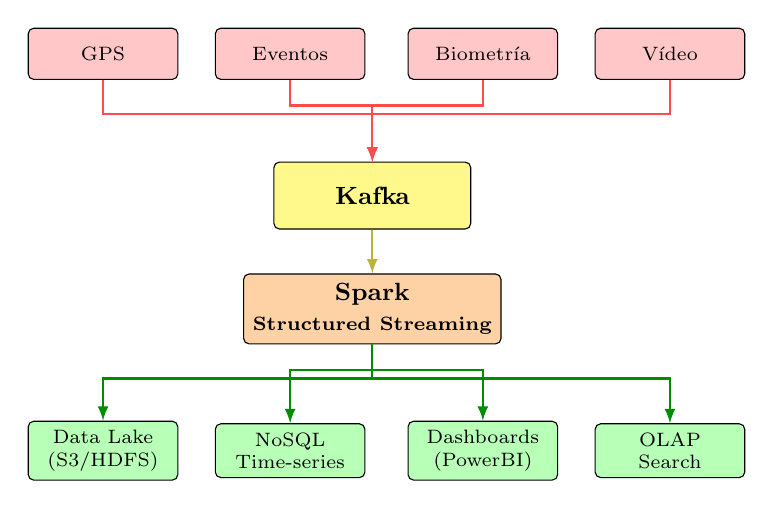
\begin{tikzpicture}[
    scale=0.72,
    source/.style={
      draw, rounded corners=2pt,
      fill=red!22, minimum width=1.9cm, minimum height=0.65cm,
      align=center, font=\scriptsize
    },
    hub/.style={
      draw, rounded corners=2pt,
      fill=yellow!45, minimum width=2.5cm, minimum height=0.85cm,
      align=center, font=\small\bfseries
    },
    proc/.style={
      draw, rounded corners=2pt,
      fill=orange!35, minimum width=2.0cm, minimum height=0.65cm,
      align=center, font=\small\bfseries
    },
    sink/.style={
      draw, rounded corners=2pt,
      fill=green!28, minimum width=1.9cm, minimum height=0.65cm,
      align=center, font=\scriptsize
    },
    >=latex
  ]

    % Sources (top row)
    \node[source] (gps)    at (-5.0,  2.5) {GPS};
    \node[source] (events) at (-1.7,  2.5) {Eventos};
    \node[source] (bio)    at ( 1.7,  2.5) {Biometría};
    \node[source] (video)  at ( 5.0,  2.5) {Vídeo};

    % Kafka hub (center)
    \node[hub]    (kafka)  at (-0.25, 0.0) {Kafka};

    % Spark (middle sink)
    \node[proc]   (spark)  at (-0.25,-2.0) {Spark\\{\scriptsize Structured Streaming}};

    % Sinks (bottom row)
      \node[sink]   (s3)     at (-5.0, -4.5) {Data Lake \\(S3/HDFS)};
      \node[sink]   (nosql)  at (-1.7, -4.5) {NoSQL \\ Time-series};
      \node[sink]   (dash)   at ( 1.7, -4.5) {Dashboards \\(PowerBI)};
      \node[sink]   (olap)   at ( 5.0, -4.5) {OLAP \\ Search};

    % Arrows: sources -> Kafka
    \draw[->, thick, red!70]   (gps.south)    -- ++(0,-0.6) -| (kafka.north);
    \draw[->, thick, red!70]   (events.south) -- ++(0,-0.45) -| (kafka.north);
    \draw[->, thick, red!70]   (bio.south)    -- ++(0,-0.45) -| (kafka.north);
    \draw[->, thick, red!70]   (video.south)  -- ++(0,-0.6) -| (kafka.north);

    % Kafka -> Spark
    \draw[->, thick, yellow!70!black] (kafka.south) -- (spark.north);

    % Spark -> sinks
    \draw[->, thick, green!55!black] (spark.south) -- ++(0,-0.6) -| (s3.north);
    \draw[->, thick, green!55!black] (spark.south) -- ++(0,-0.45) -| (nosql.north);
    \draw[->, thick, green!55!black] (spark.south) -- ++(0,-0.45) -| (dash.north);
    \draw[->, thick, green!55!black] (spark.south) -- ++(0,-0.6) -| (olap.north);

  \end{tikzpicture}
  \end{center}
\end{frame}

\begin{frame}\frametitle{Introducción - Arquitectura de referencia}
  \begin{center}
    \openvisual{Arquitectura distribuida de referencia}
    \vspace{0.2em}
    {\fontsize{5}{6}\selectfont \mbox{Fuente: \url{https://www.scaler.com/topics/spark-streaming-with-kafka/}}}
  \end{center}
\end{frame}

\begin{frame}\frametitle{Introducción - Objetivos de servicio}
\begin{itemize}
  \item \textbf{Rapidez en el análisis}
  \begin{itemize}
    \item Respuesta en tiempo real durante el partido
    \item Alertas y apoyo a decisiones en vivo
  \end{itemize}

  \vspace{1em}

  \item \textbf{Capacidad y fiabilidad del sistema}
  \begin{itemize}
    \item Procesamiento de grandes volúmenes de datos deportivos
    \item Integración de dispositivos tracking, eventos y sensores
    \item Funcionamiento estable en momentos críticos de competición
  \end{itemize}

  \vspace{1em}

  \item \textbf{Los objetivos marcan la arquitectura y los recursos}
  \begin{itemize}
    \item SLA/SLO claros para guiar decisiones
    \item Latencia objetivo y disponibilidad esperada
  \end{itemize}
\end{itemize}
\end{frame}


\begin{frame}\frametitle{Introducción - Principios de optimización}
\begin{itemize}
  \item \textbf{El cuello de botella se desplaza entre componentes}
  \begin{itemize}
    \item Optimizar un componente no garantiza mejorar todo el pipeline
    \item Al mejorar una parte la limitación suele aparecer en otra
    \item La optimización debe evaluarse a nivel global
  \end{itemize}

  \vspace{1em}

  \item \textbf{La monitorización es imprescindible}
  \begin{itemize}
    \item Comparar métricas antes y después de cada cambio
    \item Monitorizar retrasos en Kafka y tiempos en Spark
    \item Vigilar uso de recursos como disco, red y memoria
  \end{itemize}
\end{itemize}
\end{frame}


\begin{frame}\frametitle{Introducción - Principios de optimización}
\begin{itemize}

  \item \textbf{Kafka escala mejor cuando}
  \begin{itemize}
    \item Hay suficientes particiones para paralelizar producción y consumo
    \item Se añaden brokers para repartir carga y almacenamiento
    \item La infraestructura ofrece buena red y discos rápidos
  \end{itemize}

  \vspace{0.8em}

  \item \textbf{Spark escala mejor cuando}
  \begin{itemize}
    \item Hay suficiente particionado para el paralelismo de tareas
    \item Se asignan executors y memoria adecuados
    \item Se reducen los shuffles innecesarios
  \end{itemize}
\end{itemize}
\end{frame}


\section{Buenas prácticas}

% -------------------------------------------------
% Almacenamiento y datos masivos
% -------------------------------------------------

\begin{frame}\frametitle{Buenas prácticas - Análisis de datos masivos}
\begin{itemize}
  \item \textbf{Gobierno y estabilidad del dato}
  \begin{itemize}
    \item Mantener un esquema estable en pipelines críticos
    \item Definir reglas de evolución para evitar cambios incompatibles
  \end{itemize}

  \vspace{0.8em}

  \item \textbf{Organización del almacenamiento}
  \begin{itemize}
    \item Elegir un particionado coherente con las consultas más frecuentes
    \item Compactar periódicamente para mejorar el rendimiento
    \item Un buen diseño mejora el rendimiento de lectura y escritura
  \end{itemize}

  \vspace{0.8em}

  \item \textbf{Diseño según coste, latencia y tipo de procesamiento}
  \begin{itemize}
    \item En streaming se priorizan baja latencia y estabilidad operativa
    \item En batch se priorizan throughput y coste por volumen procesado
    \item Separar datos recientes (calientes) de históricos (fríos) ayuda a equilibrar ambos
  \end{itemize}
\end{itemize}
\end{frame}


\begin{frame}\frametitle{Buenas prácticas - Particionado en Kafka y Spark}
\begin{itemize}
  \item \textbf{Un buen particionado reparte la carga del pipeline}
  \begin{itemize}
    \item Nº de particiones en Kafka = paralelismo máximo de consumo
    \item En Spark cada partición se procesa como una tarea
    \item Si hay pocas particiones el clúster queda infrautilizado
  \end{itemize}

  \vspace{0.5em}

  \item \textbf{Mantiene consistencia en los datos}
  \begin{itemize}
    \item Agrupa eventos relacionados en la misma partición
    \item Conserva el orden dentro de cada partición de Kafka
  \end{itemize}

  \vspace{0.5em}

  \item \textbf{La clave debe tener suficiente granularidad}
  \begin{itemize}
    \item Claves generales concentran demasiada carga en una partición
    \item Clave más granulares mejoran el reparto y el rendimiento
    \item Ejemplos son \texttt{player\_id} o \texttt{match\_id}
  \end{itemize}
\end{itemize}
\end{frame}

% -------------------------------------------------
% Kafka: Configuración, productores y consumidores
% -------------------------------------------------

\begin{frame}
\frametitle{Buenas prácticas - Configuración en Kafka}
\begin{itemize}
  \item \textbf{Rendimiento es un equilibrio entre throughput, latencia y resiliencia}
  \begin{itemize}
    \item Depende del tamaño del mensaje, compresión y \texttt{acks}
    \item Compresión reduce tráfico de red pero añade coste de CPU
    \item \texttt{acks=all} y mayor replicación mejoran durabilidad pero aumentan latencia
  \end{itemize}

  \vspace{1em}

  \item \textbf{La infraestructura condiciona el resultado}
  \begin{itemize}
    \item Kafka es intensivo en entrada/salida $\rightarrow$ conviene usar discos rápidos
    \item La red debe ser estable y con suficiente capacidad para picos de tráfico
    \item Es buena práctica separar discos de datos y distribuir réplicas entre racks o zonas
  \end{itemize}
\end{itemize}
\end{frame}


\begin{frame}\frametitle{Buenas prácticas - Configuración en Kafka}
\begin{itemize}
  \item \textbf{Número de particiones}
  \begin{itemize}
    \item Aumentan paralelismo y throughput
    \item Demasiadas añaden overhead
  \end{itemize}

  \vspace{1em}

  \item \textbf{Factores de replicación}
  \begin{itemize}
    \item Aumenta resiliencia
    \item Aumenta el uso de disco y red
  \end{itemize}

  \vspace{1em}

  \item \textbf{Retención y compactación del log}
  \begin{itemize}
    \item Retención de mensajes $\rightarrow$ definir según su uso
    \item Compactación del log $\rightarrow$ mantiene último estado por clave
  \end{itemize}
\end{itemize}
\end{frame}

\begin{frame}\frametitle{Buenas prácticas - Replicación en Kafka}
  \begin{center}
    \openvisual{Replicación en Kafka}
    {\fontsize{5}{6}\selectfont \mbox{Fuente: \url{https://developer.confluent.io/courses/architecture/data-replication/}}}
  \end{center}
\end{frame}


\begin{frame}\frametitle{Buenas prácticas - Productores en Kafka}
\begin{itemize}
  \item \textbf{Batching para agrupar mensajes antes de enviar}
  \begin{itemize}
    \item Definir tiempo de espera para acumular más mensajes
    \item Definir tamaño máximo del batch de mensajes (bytes)
    \item Ajustes típicos son  \texttt{linger.ms} y \texttt{batch.size}
    \item Más throughput a costa de algo más de latencia de envío
  \end{itemize}

  \vspace{0.8em}

  \item \textbf{Compresión de mensajes para reducir tráfico de red y disco}
  \begin{itemize}
    \item Distintos algoritmos de compresión con diferentes trade-offs
    \item Elegir según el tamaño de los mensajes y la CPU disponible
  \end{itemize}

  \vspace{0.8em}

  \item \textbf{Fiabilidad para no perder eventos críticos}
  \begin{itemize}
    \item Definir el nivel de confirmación de escritura (\texttt{acks})
    \item Activar idempotencia para evitar duplicados por reintentos
    \item Más fiabilidad suele implicar más latencia de escritura
  \end{itemize}
\end{itemize}
\end{frame}


\begin{frame}\frametitle{Buenas prácticas - Consumidores en Kafka}
\begin{itemize}
  \item \textbf{Consumer groups para escalado horizontal}
  \begin{itemize}
    \item Añadir consumidores al mismo grupo aumenta el paralelismo
    \item El máximo útil es 1 consumidor por partición (extra quedan ociosos)
  \end{itemize}

  \vspace{0.5em}

  \item \textbf{Commits de offset para controlar el progreso}
  \begin{itemize}
    \item Los commits automáticos simplifican la configuración
    \item Los commits manuales dan más control sobre cuándo confirmar
  \end{itemize}

  \vspace{0.5em}

  \item \textbf{Reintentos y DLQs para gestionar errores}
  \begin{itemize}
    \item Definir una política de reintentos antes de descartar mensajes
    \item Enviar a una DLQ los eventos que fallan repetidamente
  \end{itemize}

  \vspace{0.5em}
  \item \textbf{Monitorizar retrasos en consumidores para detectar cuellos de botella}
\end{itemize}
\end{frame}

\begin{frame}\frametitle{Buenas prácticas - Consumer groups}
  \begin{center}
    \openvisual{Coordinación de consumidores}
    \vspace{0.2em}
    {\fontsize{5}{6}\selectfont \mbox{Fuente: \url{https://developer.confluent.io/courses/architecture/consumer-group-protocol/}}}
  \end{center}
\end{frame}


% -------------------------------------------------
% Spark: Paralelización y optimización
% -------------------------------------------------

\begin{frame}\frametitle{Buenas prácticas - Paralelización en Spark}
\begin{itemize}
  \item \textbf{Particiones, tareas y executors están relacionados}
  \begin{itemize}
    \item Spark divide los datos en particiones lógicas para procesarlos en paralelo
    \item Cada partición suele ejecutarse como una tarea independiente
    \item Los executors son los procesos que ejecutan esas tareas en los nodos del clúster
  \end{itemize}

  \vspace{0.8em}

  \item \textbf{El shuffle redistribuye datos entre nodos}
  \begin{itemize}
    \item Es habitual en operaciones como \texttt{join}, \texttt{groupBy} y agregaciones
    \item Suele ser una de las fases más costosas por uso de red, disco y tiempo
  \end{itemize}

  \vspace{0.8em}

  \item \textbf{Las particiones impactan en el rendimiento}
  \begin{itemize}
    \item Si hay pocas particiones se desaprovecha el clúster
    \item Si hay demasiadas aumenta la sobrecarga de gestión
    \item Si los executors tienen pocos recursos el procesamiento se ralentiza
  \end{itemize}
\end{itemize}
\end{frame}


\begin{frame}\frametitle{Buenas prácticas - Particionado en Spark}
\begin{itemize}
  \item \textbf{Las particiones marcan el paralelismo}
  \begin{itemize}
    \item Cada partición suele ejecutarse como una tarea por etapa
    \item Conviene ajustar su número a la capacidad real del clúster
    \item El objetivo es equilibrar paralelismo y sobrecarga
  \end{itemize}

  \vspace{0.8em}

  \item \textbf{El desbalanceo de particiones es un enemigo del rendimiento}
  \begin{itemize}
    \item Aparece cuando pocas particiones concentran muchos datos (skew)
    \item Algunas tareas terminan rápido y otras tardan mucho más
    \item El rendimiento global queda limitado por la partición más grande
    \item Primero se corrige el skew y después se ajusta el número de particiones
  \end{itemize}

  \vspace{0.8em}

  \item \textbf{Decidir entre repartir o compactar particiones}
  \begin{itemize}
    \item \texttt{repartition} $\rightarrow$ redistribuye datos con \textit{shuffle}
    \item \texttt{coalesce} $\rightarrow$ reduce particiones con menos coste (normalmente sin \textit{shuffle})
  \end{itemize}
\end{itemize}
\end{frame}


\begin{frame}\frametitle{Buenas prácticas - Skew en Spark}
  \begin{itemize}
  \item \textbf{En skew hay tareas que dominan el tiempo total del job}
  \begin{itemize}
    \item Pocas tareas lentas dominan el job (stragglers)
    \item Uso intensivo de disco mientras otros executors quedan ociosos
  \end{itemize}

  \vspace{1em}


  \item \textbf{Es clave comparar la duración de tareas en Spark}
  \begin{itemize}
    \item Si hay grandes diferencias entre tareas, suele haber desbalanceo
    \item Revisar también el tamaño de particiones tras joins y agregaciones
  \end{itemize}

  \vspace{1em}

  \item \textbf{Existen diferentes técnicas para mitigar el skew}
  \begin{itemize}
    \item Repartir mejor la carga (claves más granulares o subclaves)
    \item Tratar por separado casos con volumen anómalo
    \item Usar AQE para rebalanceo automático
  \end{itemize}
\end{itemize}
\end{frame}

\begin{frame}\frametitle{Buenas prácticas - Skew en Spark}
  \begin{center}
    \vspace{2em}
    \begin{tabular}{m{0.42\linewidth} m{0.06\linewidth} m{0.42\linewidth}}
      \centering\openvisual{Distribución de datos con skew} &
      \centering{\Large $\Rightarrow$} &
      \centering\openvisual{Distribución equilibrada}
    \end{tabular}
  \end{center}
  \begin{center}
    \vfill
    {\fontsize{5}{6}\selectfont \mbox{Fuente: \url{https://blog.scottlogic.com/2018/03/22/apache-spark-performance.html}}}
  \end{center}
\end{frame}


\begin{frame}\frametitle{Buenas prácticas - Shuffle en Spark}
\begin{itemize}
  \item \textbf{El shuffle es la operación más costosa}
  \begin{itemize}
    \item Implica serialización, red y escritura a disco intermedio
    \item Suele dominar el tiempo de ejecución en joins y agregaciones
  \end{itemize}

  \vspace{0.8em}

  \item \textbf{Reducir datos antes del shuffle}
  \begin{itemize}
    \item Filtrar filas y proyectar solo las columnas necesarias
    \item Preagregar cuando sea posible antes de un join
    \item Menos datos en movimiento implica menos coste y menor latencia
  \end{itemize}

  \vspace{0.8em}

  \item \textbf{Usar broadcast join con tablas pequeñas}
  \begin{itemize}
    \item Si una tabla cabe en memoria, se copia a los executors
    \item Así se evita redistribuir la tabla grande
    \item Genera menos shuffle y joins más rápidos
  \end{itemize}
\end{itemize}
\end{frame}

\begin{frame}\frametitle{Buenas prácticas - Shuffle en Spark}
  \begin{center}
    \openvisual{Operación de shuffle}
  \end{center}
  \begin{center}
      {\fontsize{5}{6}\selectfont \mbox{Fuente: \url{https://blog.scottlogic.com/2018/03/22/apache-spark-performance.html}}}
  \end{center}
\end{frame}



\begin{frame}\frametitle{Buenas prácticas - Caching en Spark}
\begin{itemize}
  \item \textbf{Guarda datos intermedios para reutilizarlos}
  \begin{itemize}
    \item Solo compensa cuando esos datos se usan varias veces
    \item Si un resultado se usa una sola vez suele empeorar el rendimiento
  \end{itemize}

  \vspace{1em}

  \item \textbf{La cache ocupa memoria y compite con la ejecución de tareas}
  \begin{itemize}
    \item Si no hay memoria suficiente aumenta el uso de disco y baja el rendimiento
    \item Conviene priorizar datasets intermedios costosos y estables
  \end{itemize}

  \vspace{1em}

  \item \textbf{Buenas prácticas de uso}
  \begin{itemize}
    \item Cachear después de transformaciones costosas que se reutilizan
    \item Liberar el cache cuando deja de ser necesario y validar impacto con métricas
  \end{itemize}
\end{itemize}
\end{frame}


\begin{frame}\frametitle{Buenas prácticas - Persistencia y checkpointing en Spark}
\begin{itemize}
  \item \textbf{Persistir extiende la idea de cache}
  \begin{itemize}
    \item El cache es una forma de persistencia en memoria
    \item La persistencia permite elegir cómo guardar los datos
    \item Se usa cuando el mismo DataFrame se reutiliza y el volumen puede ser alto
  \end{itemize}

  \vspace{0.8em}

  \item \textbf{Existen varios niveles de persistencia}
  \begin{itemize}
    \item \texttt{MEMORY\_ONLY} $\rightarrow$ más rápido si los datos caben en memoria
    \item \texttt{MEMORY\_AND\_DISK} $\rightarrow$ más robusto cuando el volumen es grande
  \end{itemize}

  \vspace{0.8em}

  \item \textbf{Checkpointing para análisis en streaming}
  \begin{itemize}
    \item Guarda el estado del pipeline para recuperarse tras fallos
    \item Es clave en ventanas temporales, deduplicación y joins con estado
    \item Debe guardarse en almacenamiento fiable (HDFS, S3 o equivalente)
  \end{itemize}
\end{itemize}
\end{frame}




\section{Puesta en producción}


\begin{frame}\frametitle{Puesta en producción - Kafka en on-premises}
\begin{itemize}
  \item \textbf{Elegir el modelo de despliegue}
  \begin{itemize}
    \item Bare metal prioriza rendimiento y control de la infraestructura
    \item Máquinas virtuales ofrecen más flexibilidad con algo de sobrecarga
    \item Kubernetes facilita la operación pero exige cuidar el almacenamiento persistente
  \end{itemize}

  \vspace{0.5em}

  \item \textbf{Kafka depende mucho del rendimiento de disco y de red}
  \begin{itemize}
    \item Conviene usar almacenamiento rápido para los logs
    \item También es importante una red estable entre brokers
  \end{itemize}

  \vspace{0.5em}

  \item \textbf{Es fundamental asegurar la continuidad del servicio}
  \begin{itemize}
    \item Se recomiendan al menos 3 brokers y factor de replicación 3 en tópicos críticos
    \item Distribuir réplicas en distintos nodos o racks mejora la disponibilidad
    \item KRaft simplifica el despliegue frente a ZooKeeper
  \end{itemize}

  \vspace{0.5em}

  \item \textbf{Dimensionar almacenamiento y límites de mensajes}
\end{itemize}
\end{frame}


\begin{frame}\frametitle{Puesta en producción - Spark en on-premises}
\begin{itemize}
  \item \textbf{Conviene elegir el gestor del clúster según el entorno}
  \begin{itemize}
    \item YARN encaja bien en ecosistemas Hadoop
    \item Kubernetes facilita orquestación, aislamiento y elasticidad
    \item Spark standalone suele reservarse para desarrollo y pruebas
  \end{itemize}

  \vspace{0.8em}

  \item \textbf{El almacenamiento condiciona el rendimiento y la operación}
  \begin{itemize}
    \item HDFS es una opción sólida para cargas batch
    \item Checkpointing debe guardarse en almacenamiento fiable
  \end{itemize}

  \vspace{0.8em}

  \item \textbf{Es importante separar cargas y fijar dependencias}
  \begin{itemize}
    \item Conviene separar recursos de batch y streaming
    \item Streaming necesita mayor prioridad para mantener la latencia
    \item Docker ayuda a mantener dependencias y versiones estables
  \end{itemize}
\end{itemize}
\end{frame}


\begin{frame}\frametitle{Puesta en producción - Kafka en AWS}
\begin{itemize}
  \item \textbf{Conviene elegir entre servicio administrado y control directo}
  \begin{itemize}
    \item Amazon MSK es Kafka administrado por AWS y reduce trabajo de operación
    \item MSK Serverless ajusta recursos automáticamente cuando la carga cambia
    \item Kafka en EC2 da más control de configuración pero exige más operación
  \end{itemize}

  \vspace{1em}

  \item \textbf{La red y el acceso se controlan dentro de AWS}
  
  \vspace{1em}

  \item \textbf{Seguridad y monitorización deben configurarse desde el inicio}
  \begin{itemize}
    \item IAM puede gestionar autenticación y autorización de clientes
    \item CloudWatch centraliza métricas para monitorizar brokers, tópicos y consumo
  \end{itemize}
\end{itemize}
\end{frame}


\begin{frame}\frametitle{Puesta en producción - Spark en AWS}
\begin{itemize}
  \item \textbf{Conviene elegir la plataforma según el tipo de carga}
  \begin{itemize}
    \item Amazon EMR encaja bien en batch y en streaming
    \item Spark sobre EKS aporta flexibilidad y encaje con contenedores
    \item Databricks en AWS simplifica desarrollo y operación
  \end{itemize}

  \vspace{1em}

  \item \textbf{En AWS Spark se suele lanzar como jobs}
  \begin{itemize}
    \item Como EMR Steps, \texttt{spark-submit} en EKS o Jobs en Databricks
  \end{itemize}

  \vspace{1em}

  \item \textbf{Es importante diferenciar el uso en streaming y en batch}
  \begin{itemize}
    \item Un flujo habitual conecta MSK o Kinesis con Spark Structured Streaming
    \item En streaming se priorizan latencia y estabilidad del pipeline
    \item En batch se priorizan throughput y coste por volumen procesado
  \end{itemize}
\end{itemize}
\end{frame}


\begin{frame}\frametitle{Puesta en producción - Monitorización en Kafka}
\begin{itemize}
  \item \textbf{La monitorización debe centrarse en la salud del pipeline}
  \begin{itemize}
    \item El retraso del consumidor es la métrica principal para detectar retraso
    \item También conviene seguir la tasa de producción y consumo por tópico
    \item La latencia de extremo a extremo ayuda a comprobar si se cumplen los objetivos
  \end{itemize}

  \vspace{0.8em}

  \item \textbf{La replicación y el disco son claves para la estabilidad}
  \begin{itemize}
    \item Problemas en el ISR pueden señalar riesgo de pérdida o menor disponibilidad
    \item El uso de disco por broker debe vigilarse de forma continua
  \end{itemize}

  \vspace{0.8em}

  \item \textbf{Las alertas y herramientas deben adaptarse al entorno}
  \begin{itemize}
    \item Configurar alertas por consumer lag, timeouts y errores de broker
    \item En on-premises es habitual usar Prometheus y Grafana
    \item En AWS se suele usar CloudWatch y métricas de MSK
  \end{itemize}
\end{itemize}
\end{frame}

\begin{frame}\frametitle{Puesta en producción - Monitorización en Kafka}
  \begin{center}
    \openvisual{Observabilidad de Kafka}
    \vspace{0.1em}
    {\fontsize{5}{6}\selectfont \mbox{Fuente: \url{https://grafana.com/blog/get-comprehensive-monitoring-for-your-apache-kafka-ecosystem-instances-quickly-with-grafana-cloud/}}}
  \end{center}
\end{frame}



\begin{frame}\frametitle{Puesta en producción - Monitorización en Spark}
\begin{itemize}
  \item \textbf{Spark Web UI permite localizar cuellos de botella}
  \begin{itemize}
    \item En la vista de \textit{stages} se ve qué etapas concentran más tiempo
    \item Dentro de cada etapa las \textit{tasks} permiten comparar duraciones y detectar skew
    \item Las métricas de \textit{shuffle read/write} muestran cuánto dato se mueve entre nodos
  \end{itemize}

  \vspace{0.8em}

  \item \textbf{En streaming hay que vigilar el ritmo del pipeline}
  \begin{itemize}
    \item La duración del micro-batch debe ser menor que el intervalo del trigger
    \item Comparar datos que entran y datos que se procesan ayuda a ver retrasos
    \item Los registros pendientes muestran si se está acumulando trabajo
    \item Medir tasa de input y procesamiento, duración del batch y watermark
  \end{itemize}

  \vspace{0.8em}

  \item \textbf{Las alertas deben avisar antes de que el pipeline falle}
  \begin{itemize}
    \item Alertar si aumenta el uso de disco o el tiempo de limpieza de memoria
    \item Alertar de inmediato ante jobs fallidos con contexto del error
  \end{itemize}
\end{itemize}
\end{frame}

\begin{frame}\frametitle{Puesta en producción - Monitorización en Spark}
  \begin{center}
    \openvisual{Interfaz de monitorización de Spark}
    \vspace{0.2em}
    {\fontsize{5}{6}\selectfont \mbox{Fuente: \url{https://spark.apache.org/docs/latest/web-ui.html}}}
  \end{center}
\end{frame}



\begin{frame}{Fuentes, imágenes y reutilización}
\small
\begin{itemize}
  \item El texto, los ejemplos y los esquemas de esta edición abierta se distribuyen bajo CC BY-SA 4.0.
  \item Las imágenes de procedencia no acreditada de la versión de trabajo se han retirado y sustituido por esquemas conceptuales originales.
  \item Los logotipos y marcas citados se utilizan únicamente con finalidad identificativa y quedan excluidos de la licencia.
  \item Las referencias técnicas se conservan mediante citas y enlaces a sus fuentes correspondientes.
  \item Información de licencia: \url{https://creativecommons.org/licenses/by-sa/4.0/deed.es}
\end{itemize}
\end{frame}

\end{document}
